\documentclass[preprint,12pt]{elsarticle}
\usepackage[T1]{fontenc}
\usepackage[utf8]{inputenc}
\usepackage{lmodern}
\usepackage{microtype}
\usepackage{amsmath,amssymb}
\usepackage{booktabs,tabularx,array,longtable}
\usepackage{graphicx}
\usepackage{url}
\usepackage[hidelinks]{hyperref}
\emergencystretch=2em
\journal{Journal of Information Security and Applications}

\begin{document}
\begin{frontmatter}
\title{A Multi-Axis Empirical Audit of Machine-Learning Intrusion Detection}
\author[anon]{AUTHOR\_CONFIRMATION\_REQUIRED}
\address[anon]{AUTHOR\_CONFIRMATION\_REQUIRED}
\begin{abstract}
Conventional machine-learning intrusion-detection benchmarks provide useful controlled comparisons, but their discrimination metrics do not alone establish validity across chronology, operating points, datasets, prevalence, computational paths, or attack families withheld from development. We conducted a bounded, source-faithful empirical validity audit centered on CSE-CIC-IDS2018, with a restricted CICIDS2017 bridge. The audit separated processed-reference evaluation from source-faithful temporal and transfer populations and examined frozen operating-point transfer, registered feature and explanation sensitivity, direction-specific semantic bridges, analytic prevalence and workload projections, component-level computational profiling, eligible leave-one-attack-family-out evaluation, and finite-seed stability. On the processed reference holdout, balanced XGBoost achieved F1 0.9285 and PR-AUC 0.9776. On one shared forward target, chronological-natural development produced mean PR-AUC 0.6388 versus 0.2599 after random-natural development across five registered realizations; the ordering was descriptive and held in all five, while frozen thresholds transferred poorly. Bridge62 transfer was directional: PR-AUC was 0.667483 from IDS2018 to CICIDS2017 and 0.108176 in the reverse direction. Under an analytic 0.1\% prevalence scenario, projected PPV and analyst workload diverged, including PPV 0.965572 with 33.5 analyst-hours per day for one point. Eligible-family behavior was selective, and computational feasibility was specific to measured compatible paths and hardware. These findings show that IDS conclusions depend on population, protocol, representation, operating rule, and evidence status; they do not establish universal deployment readiness, zero-day detection, temporal causation, or complete historical reproduction.
\end{abstract}
\begin{keyword}
Network intrusion detection \sep temporal validation \sep cross-dataset generalization \sep operating-point transfer \sep attack-family evaluation \sep reproducibility
\end{keyword}
\end{frontmatter}


\section{Introduction}

Machine-learning intrusion-detection benchmarks provide useful controlled evidence. A fixed population, representation, learner, and decision rule can support reproducible comparison of discrimination and operating behavior. Such evidence should not be discarded because it is conditional. It answers a narrower question: how well does a fitted detector separate the labels in the evaluated benchmark under the declared protocol? Network intrusion detection, however, is applied to traffic whose chronology, collection environment, feature contract, prevalence, attack composition, and computational path may differ from those conditions \cite{sommer2010closed,ring2019survey,arp2022dos}.

Consequently, strong benchmark discrimination does not by itself establish future-facing reliability. Ranking metrics describe score ordering, whereas a deployed decision rule depends on a threshold, calibration, prevalence, and action cost \cite{saito2015precision,axelsson2000baserate}. Cross-dataset evidence additionally depends on source-to-target direction, semantic feature correspondence, preprocessing, and target construction \cite{dhooge2020interdataset,layeghy2023crossdomain}. Feature ablations and explanations can reveal sensitivity, but neither feature removal nor attribution repeatability alone identifies a causal shortcut or faithful local reasoning \cite{engelen2021troubleshooting,arp2022dos,ribeiro2016lime,lundberg2017shap,yeh2019infidelity}. Operational interpretation requires alert volume, workload, yield, and assumptions about base rates; computational claims require a declared hardware and software boundary. Finally, withholding an attack family is more demanding than evaluating known categories, but its interpretation remains dependent on eligibility, support, learner, metric, and threshold.

These quantities should remain separate. A model may rank a forward target better while its inherited threshold transfers poorly. A direction may retain cross-dataset ranking while the reciprocal direction is near its prevalence and chance anchors. High projected positive predictive value may coexist with a burdensome alert stream, while low workload may reflect negligible detection yield. Such tensions are not one-dimensional robustness failures; they define the conditions under which each inference is informative.

Prior research has already established important parts of this evaluation problem. Dataset audits document extraction errors, artifacts, and dependence concerns in widely used intrusion-detection benchmarks \cite{engelen2021troubleshooting,arp2022dos}. Time-aware evaluation provides a future-use direction, while work on experimental bias shows that split geometry and collection order can change the interpretation of machine-learning results \cite{pendlebury2019tesseract}. Cross-dataset studies examine transfer strength, shared representations, and domain dependence \cite{dhooge2020interdataset,layeghy2023crossdomain,cantone2024crossdataset}. Explainability research provides tools such as LIME, SHAP, and TreeSHAP, together with separate concepts of sensitivity and fidelity \cite{ribeiro2016lime,lundberg2017shap,lundberg2020trees,yeh2019infidelity}. Base-rate analysis and prior-probability adjustment explain why discrimination and positive predictive value cannot be interpreted independently \cite{axelsson2000baserate,saerens2002prior}. Open-set and unknown-attack studies likewise provide established protocols for testing behavior beyond development classes \cite{scheirer2013openset,zoppi2023unknown,shin2023openset}.

Recent work makes the overlap with the present study especially direct. Berhili, Chaieb, and Benabdellah investigate protocol-dependent inflation across three datasets, with documented analyses of validation-split bias, seed sensitivity, preprocessing leakage, semantically aligned transfer, calibration, threshold choices, statistical testing, and reproducibility artifacts \cite{berhili2026protocol,berhili2026reproducibility}. Their article-level access was incomplete in the present review, so uninspected dimensions are not treated as omissions. Biswas reports a non-peer-reviewed preprint using CSE-CIC-IDS2018 and CIC-DDoS2019 to compare random, stratified-temporal, and class-blind chronological protocols, cross-regime transfer, calibration, and unseen-family interpretation \cite{biswas2026drift}. This work directly establishes the relevance of temporal-protocol sensitivity on IDS2018; the present study therefore makes no conceptual-priority claim for temporal validation or unseen-family testing.

Elangovan et al. study temporal and semantic cross-dataset generalization across four public datasets \cite{elangovan2026crossdataset}. Mishra et al. report harmonized cross-dataset multi-model learning with statistical validation \cite{mishra2026harmonized}; their associated correction concerns the funding statement, not the methodology or results \cite{mishra2026correction}. Ha Thanh's TAN-IDS frames transfer-aware, deployment-oriented evaluation around NetFlow representation and adaptation scenarios \cite{hathanh2026tanids}. Buriboyev reports a factorial protocol audit on CICIDS2017 involving temporal partitioning, shortcut-related factors, protocol interactions, and ranking instability, but its Zenodo record and linked article copy do not independently establish peer-reviewed publication status \cite{buriboyev2026protocol}. These studies make clear that the relevant evaluation dimensions and several of their combinations are prior art.

The remaining problem is narrower: how should a linked, source-faithful chain of study-specific evidence be interpreted when its evaluation contracts change across population, chronology, threshold, representation, transfer direction, prevalence, hardware, attack-family eligibility, and model realization? This is not a gap created by the absence of temporal validation, semantic alignment, explainability, LOAO, or reproducibility practice. It is an interpretation problem concerning which observations survive, which become conditional, which planned cells are unavailable, and which claims must stop at the artifact boundary.

This study addresses that problem through a bounded audit centered on CSE-CIC-IDS2018 and a restricted CICIDS2017 bridge. The processed and stratified reference remains a conventional baseline. Separately governed source-faithful temporal populations, frozen operating points, registered feature and placebo controls, direction-specific semantic bridges, analytic prevalence/workload translations, component-level profiling, eligible LOAO, and finite-seed closure are treated as different estimands. The resulting contribution is the documented empirical pattern and its interpretation ceilings, not the invention of a new evaluation framework. Numerical findings are deferred to the Results and are not used here to imply portability beyond the evaluated contracts.

The audit addresses six questions:

1. \textbf{Benchmark and forward validity:} How does discrimination under the processed CSE-CIC-IDS2018 reference relate to ranking on the separately governed forward target?
2. \textbf{Ranking and decision transfer:} Do ranking changes under random versus chronological development transfer to the frozen operating points selected during development?
3. \textbf{Representation and explanation sensitivity:} How do registered feature subsets, split geometry, learner realization, TreeSHAP comparison, and LIME fidelity change the interpretation of feature reliance?
4. \textbf{Directional transfer:} Does ranking transfer symmetrically between CSE-CIC-IDS2018 and CICIDS2017 under the frozen bridge62 and bridge70 contracts?
5. \textbf{Operational and computational interpretation:} How do assumed prevalence, workload, cost, and the measured component-level hardware boundary alter the meaning of discrimination and threshold results?
6. \textbf{Eligibility and realization stability:} What behavior remains under eligible leave-one-attack-family-out evaluation and the registered finite-seed/control program?

Each question is answered only by the frozen stages mapped in the crosswalk supplied with this section. None requires a new fit, target opening, threshold search, statistical test, or scientific recomputation.

The study makes three linked, bounded contributions.

\textbf{1. Protocol-conditioned empirical findings.} The audit reports source-faithful temporal and frozen-operating-point results, registered shortcut and placebo controls, finite-seed stability, and direction-specific semantic transfer. The relevant Stage 29 claims are \texttt{CLM29-005}, \texttt{CLM29-008}--\texttt{CLM29-011}, and \texttt{CLM29-016}, supported by \texttt{E29-016}, \texttt{E29-020}--\texttt{E29-027}, and \texttt{E29-037}--\texttt{E29-040}. Chronological development ranked higher on the shared forward target across the five registered realizations, but frozen thresholds transferred poorly; shortcut effects varied by split and learner; transfer was directional. The chronology/family-composition confounding, historical target reuse, K79 exact-identity boundary, cancelled \texttt{GROUNDED\_S4} cells, and failure to isolate one causal mechanism prevent claims of universal temporal superiority, concept drift, causal shortcut explanation, or symmetric portability.

\textbf{2. Operational and eligibility-gated stress tests.} The study complements those findings with analytic prevalence/workload projections, frozen operating-point utility, component-level profiling, and eligible-family LOAO. Claims \texttt{CLM29-013}--\texttt{CLM29-015}, supported by \texttt{E29-028}--\texttt{E29-039}, show that PPV, alert burden, yield, cost, measured computation, and withheld-family behavior can diverge. Profiling covers compatible prepared-input-to-probability paths on recorded hardware and software; unsupported paths remain unsupported. LOAO excludes DOS and AUTH\_BRUTE\_FORCE, while Infiltration has 36 held-out positives and remains descriptive; known-category \texttt{Infilteration} support of 3,967 is a different population. These results are analytic or benchmark-bound evidence, not SOC observations, end-to-end latency, universal zero-day detection, or production readiness.

\textbf{3. Evidence-governed interpretation.} Claim-to-artifact provenance, target-opening records, incomplete historical reproducibility, cancelled-cell governance, and unsupported-path statuses make the evidence boundary inspectable. \texttt{CLM29-012} and \texttt{CLM29-014}--\texttt{CLM29-016}, together with \texttt{LIM29-001}--\texttt{LIM29-018}, document what is directly demonstrated, supported, descriptive, cancelled, unavailable, or unsupported. This is a transparency contribution built on established reproducibility practice, not a wholly new methodology or independent rerun. Static and scalar verification do not imply complete end-to-end regeneration.

Section 2 reviews benchmark and temporal protocols, feature and explanation validity, transfer and operational evaluation, and computational, unseen-family, and reproducibility concerns. Section 3 defines the datasets, provenance, populations, bridges, family eligibility, and target governance. Section 4 describes the frozen evaluation contracts and metrics. Section 5 reports the empirical results. Section 6 interprets the findings against their validity boundaries. Section 7 states threats to validity and unresolved evidence limitations. Section 8 concludes with the bounded implications for IDS evaluation.

\section{Related Work}

Benchmark datasets remain valuable because they make model comparisons possible under shared labels, features, and evaluation procedures. Surveys of network-based intrusion-detection datasets also show why those comparisons are conditional on collection design, labeling, representation, and class construction \cite{ring2019survey}. The CSE-CIC-IDS2018 and CICIDS2017 releases provide important flow-derived resources \cite{sharafaldin2018toward,cse_cic_ids2018_official,cicids2017_official}, but a processed or rebalanced table should not be treated as a natural deployment population. Imbalanced-learning guidance and precision-recall analysis further motivate reporting native quantities appropriate to the evaluated class distribution \cite{he2009imbalanced,saito2015precision}.

Security-dataset audits have documented extraction errors, duplicate-like relationships, and collection artifacts that complicate random partitioning \cite{engelen2021troubleshooting,arp2022dos}. Time-aware evaluation addresses a different question: whether a model trained under an earlier role can rank a later population. Work on experimental bias across space and time shows that partition geometry can change reported results \cite{pendlebury2019tesseract}. Yet chronology can also change attack-family composition and prevalence. A chronological contrast therefore identifies behavior under a chosen forward contract; it does not, on its own, prove concept drift or establish that chronological development is universally superior.

The most direct recent comparisons are Berhili et al. and Biswas. Berhili et al. study protocol-dependent accuracy inflation across UNSW-NB15, NSL-KDD, and CICIDS2017. Their accessible implementation and package document validation-split comparisons, seed sensitivity, preprocessing leakage, semantically aligned transfer, calibration and threshold analyses, statistical testing, and reproducibility artifacts \cite{berhili2026protocol,berhili2026reproducibility}. The article and supplement were not fully accessible for this review; consequently, dimensions not independently inspected remain unverified rather than absent. Biswas's 2026 Preprints.org record is explicitly a non-peer-reviewed preprint \cite{biswas2026drift}. It examines CSE-CIC-IDS2018 under random, class-stratified temporal, and class-blind chronological protocols, then studies cross-regime transfer and target calibration with an unseen-family framing. Its temporal-protocol evidence makes the conceptual problem directly prior to the present study. Buriboyev likewise reports a four-factor CICIDS2017 protocol audit with temporal partitioning, shortcut-related factors, interactions, and ranking instability, but Zenodo resource metadata and a linked article copy do not independently verify peer-reviewed venue status \cite{buriboyev2026protocol}.

The present audit therefore does not claim to introduce temporal validation or protocol-bias analysis. Its narrower empirical question is how the frozen CSE-CIC-IDS2018 development contracts behave on one source-faithful forward target when ranking and operating-point transfer are reported separately, when feature interventions and controls are retained, and when finite-seed stability is distinguished from causal or population inference. The K79 control establishes exact corrected-second-plus-predictor identity under its declared rule; it does not establish session, endpoint, source-IP, five-tuple, or S4 independence. The temporal target was historically opened and later reused for registered stability analysis, so that analysis is not a new blind holdout.

A detector can exploit fields that are predictive in one collection protocol without encoding behavior that transports to another. Dataset troubleshooting and broader computer-security evaluation guidance therefore motivate inspection of identifiers, extraction fields, collection artifacts, and feature dependencies \cite{engelen2021troubleshooting,arp2022dos}. Cross-dataset work reinforces the importance of a semantic feature contract: shared names or positional overlap are not sufficient evidence that two variables represent the same construct \cite{dhooge2020interdataset,layeghy2023crossdomain}.

Feature ablation is useful but limited. Removing a registered field or subset measures sensitivity to that intervention under the tested split and learner. It does not prove that the field is leakage, that it caused transfer failure, or that the observed mechanism is causal. Matched-size placebos, stump probes, proxy-absorption checks, and family-support records can constrain interpretations, but observational controls may still leave multiple mechanisms compatible with the result. The present study follows this boundary: its shortcut claims are conditional sensitivity findings, and its Stage 28 controls did not isolate one causal temporal or family-composition mechanism.

Explanation methods provide another, distinct diagnostic. LIME constructs a local surrogate explanation for a prediction \cite{ribeiro2016lime}. SHAP formalizes additive feature attribution, while TreeSHAP provides a tree-specific implementation \cite{lundberg2017shap,lundberg2020trees}. Research on explanation infidelity and sensitivity cautions that stable or plausible attributions need not be faithful to the underlying decision function \cite{yeh2019infidelity}. Accordingly, explanation stability, model-decision reproduction, local surrogate fidelity, and agreement between attribution rankings are separate properties.

The present audit uses that separation. TreeSHAP agreement across the two tree learners is descriptive attribution evidence. The deterministic LIME panel tests local behavior against explicit criteria; repeatability across perturbation seeds does not override local decision failures. Integrated Gradients and attention analyses remain bounded to their documented neural-model contexts and are not generalized into a common explanation for all branches. The empirical contribution is therefore a documented representation-and-explanation sensitivity pattern under registered subsets and criteria, not a new explainability method or causal account of shortcut use.

Cross-dataset IDS studies show that transfer depends on dataset pairing, representation, preprocessing, source-to-target direction, and the target population \cite{dhooge2020interdataset,layeghy2023crossdomain,cantone2024crossdataset}. Elangovan et al. extend this line with temporal and semantic generalization across four public datasets, including forward and cross-domain comparisons \cite{elangovan2026crossdataset}. Mishra et al. study harmonized cross-dataset multi-model learning with statistical validation \cite{mishra2026harmonized}. The correction associated with that article concerns its funding statement and is not a methodology or results correction \cite{mishra2026correction}. Ha Thanh's TAN-IDS frames transfer in a unified NetFlow representation with adaptation and deployment-oriented scenarios \cite{hathanh2026tanids}. Adaptation-oriented evaluation and source-only transfer answer different questions; neither is treated here as generally superior.

Berhili et al. provide especially close prior evidence by documenting semantic alignment, bidirectional transfer, and deployable-versus-oracle calibration in their accessible implementation \cite{berhili2026protocol}. Biswas reports cross-regime zero-shot transfer and target calibration in the non-peer-reviewed preprint record \cite{biswas2026drift}. These studies prevent a claim that semantic alignment, cross-dataset transfer, calibration, or operating-point analysis is newly invented. The present study instead preserves source and target roles under frozen bridge contracts. Bridge62 and bridge70 are not interchangeable: bridge62 excludes the eight aggregate flag-count fields, whereas bridge70 retains the aggregate fields and compares published with corrected serialization. The two directions are reported separately, not averaged into a portability score. The two planned \texttt{GROUNDED\_S4} cells were cancelled before target opening because durable physical-row membership could not be recovered without a new heuristic; they are no-result administrative conditions, not negative model findings.

Operational interpretation begins with the base-rate problem. Sensitivity and specificity do not determine positive predictive value when attacks are rare \cite{axelsson2000baserate}. Prior-probability-shift methods can translate classifier outputs to new class priors, but their interpretation depends on assumptions about stable class-conditional behavior \cite{saerens2002prior}. Controlled human-factors work also demonstrates that false-alarm rate can affect analyst performance and time on task \cite{layman2023falsealarms}. Thus PPV, alert volume, analyst-hours, detection yield, capacity, and cost should not be collapsed into one favorable metric. The present Stage25 quantities are deterministic projections under fixed TPR/FPR, assumed prevalence, traffic volume, service time, analyst capacity, and relative costs. They are not observed SOC workload, organization-specific economics, or production utility.

Computational results are meaningful only at a declared boundary. Benchmarking practice emphasizes that timing depends on implementation, hardware, batch, and measurement procedure \cite{mattson2020mlperf}. Online IDS systems also illustrate the importance of distinguishing feature extraction and stream processing from model inference \cite{mirsky2018kitsune}. The present component-level profiling begins with prepared model input and ends with materialized probabilities on recorded CPU/Tesla-T4 environments. Packet capture, flow extraction, feature construction, representation conversion, alert aggregation, transport, and analyst response are outside the timed boundary. Unsupported backends, timeouts, and resource-limited paths remain statuses; they are not converted into poor timings. The results therefore establish measured compatibility and feasibility for the recorded paths, not end-to-end latency or hardware-independent architecture superiority.

Unknown-attack evaluation has established conceptual links with open-set recognition and supervised, unsupervised, and meta-learning approaches to unknown attacks \cite{scheirer2013openset,zoppi2023unknown,shin2023openset}. In IDS, however, unseen is protocol-specific. A valid LOAO condition requires zero exposure to the held-out family in training and validation, a declared chronology, sufficient target support, and a clear distinction between ranking and threshold behavior. The present eligibility gates exclude DOS and AUTH\_BRUTE\_FORCE; Infiltration is executable but descriptive with 36 held-out positives. This must not be conflated with the known-category \texttt{Infilteration} support of 3,967 in the processed reference. The resulting evidence is selective family- and learner-dependent behavior, not universal zero-day detection.

Statistical and realization controls answer different questions. Conditional bootstrap intervals describe uncertainty for frozen populations and arrays; five registered seeds describe finite model-realization stability. Neither becomes a population guarantee merely by being reported together. The Stage28 ordering is descriptive over five seeds, and family-level behavior remains heterogeneous.

Reproducibility work emphasizes code, experimental detail, and regeneration \cite{pineau2021reproducibility}. Berhili's package is a relevant example: it supplies code, scripts, indices, seeds, and result files, while datasets remain external \cite{berhili2026reproducibility}. The present evidence-governance layer should be read in that context. Claim-to-artifact mappings, target-opening records, equivalence receipts, cancellation records, and unsupported-path statuses make this study's evidence boundaries inspectable. They do not constitute a wholly new reproducibility methodology or prove complete rerun equivalence. Historical source data, models, arrays, and environments remain heterogeneous in availability; static verification and deterministic scalar checks are not the same as full scientific regeneration.

Taken together, prior work establishes the relevant evaluation tools and many close protocol questions. The present paper is positioned more narrowly as a source-faithful empirical validity audit of CSE-CIC-IDS2018 and a restricted CICIDS2017 bridge. Its empirical positioning rests on the particular frozen observations and interpretation ceilings reported across temporal ranking, operating-point transfer, feature and explanation sensitivity, directional transfer, analytic workload, measured computation, eligible-family behavior, and evidence status. These observations are bounded by the stated populations, bridges, supports, historical target reuse, finite seeds, cancelled cells, and incomplete reproducibility; they do not establish methodological priority or universal IDS behavior.

\section{Datasets and Provenance}

\subsection{3.1 CSE-CIC-IDS2018 roles}
CSE-CIC-IDS2018 serves two non-equivalent roles \cite{cse_cic_ids2018_official, sharafaldin2018toward}. The conventional reference uses the original processed, rebalanced binary table, with frozen memberships of 192,593 training, 48,149 validation, and 60,186 holdout rows. It supports controlled model and operating-point selection but is not a natural-prevalence, session-independent, or forward population.
Recovered temporal provenance showed that the inherited membership was unsafe for temporal-window evaluation. Temporal analyses therefore use source-faithful dated exports and separately governed memberships. Here, source-faithful means that authenticated columns, cleaning rules, and temporal roles were recovered from the research lineage; it does not imply raw-packet availability or complete reconstruction of every historical environment. The shared forward target preserves collection order and is scientifically distinct from the processed holdout. High reference discrimination is not relabeled as temporal evidence, and the source-faithful analysis does not make the processed reference naturalistic.

\subsection{3.2 CICIDS2017 and semantic bridges}
CICIDS2017 supplies a second benchmark domain, selected packet/flow provenance, and the family/day chronology used for LOAO evaluation \cite{cicids2017_official, sharafaldin2018toward}. The primary forward bridge trains on IDS2018 and evaluates 2,830,743 effective CICIDS2017 rows; the reverse bridge trains under the frozen CICIDS2017 source protocol and evaluates the IDS2018 February 28 target. The directions are not averaged because their learners, prevalence, representations, and target roles differ.
Cross-dataset comparability follows frozen semantic contracts. Bridge62 contains the defensible shared predictors. Bridge70 adds aggregate-flag fields and retains both the published serialization and a preregistered correction. The correction changes an identified representation dependency; it is not selected after target performance. Two planned \texttt{GROUNDED\_S4} cells were cancelled before target opening because exact durable physical-row membership could not be reconstructed without a new heuristic. They were neither approximated nor replaced.

\subsection{3.3 Attack-family populations}
Known categories in the processed reference holdout describe error concentration, not novelty. LOAO evaluation instead requires zero exposure to the target family in training and validation, a day-atomic \texttt{TRAIN < VALIDATION < TARGET} ordering, and sufficient target support. DDoS, Port Scan, Web Attack, Bot, and Infiltration were eligible. DOS and AUTH\_BRUTE\_FORCE were structurally ineligible, while Infiltration remained descriptive because its target contained 36 positives. The primary family target pairs the withheld family with temporally matched benign traffic; a context target that includes known attacks remains secondary.

\subsection{3.4 Provenance and target governance}
Provenance labels retain narrow meanings. \texttt{Raw-exact} denotes preserved source bytes; \texttt{published} denotes released artifact semantics; \texttt{corrected} denotes a frozen documented correction; \texttt{source-faithful} denotes a derived representation following authenticated semantics and locked cleaning; and \texttt{reconstructed} denotes recovery from surviving lineage evidence without claiming byte identity. Detailed parser investigations, transport receipts, storage events, and failed mechanism searches are routed to the supplement or repository unless needed to interpret a main result.
Development data support fitting, validation selection, and protocol checks only within declared roles. Target-facing model scope, features, thresholds, and cleaning were frozen before the corresponding target result. No target-guided fitting, feature search, calibration, or threshold reselection occurred. Some targets were historically opened and later reused for preregistered stability analysis; they are not presented as fresh blind holdouts. Current validation-safe interfaces verify identities, schemas, values, and receipts without opening scientific targets or deserializing models.

\section{Validation Framework and Methods}

\subsection{4.1 Reference evaluation}
The reference question is conventional within-table discrimination on the processed CSE-CIC-IDS2018 binary data. Stratified training, validation, and holdout memberships are frozen and disjoint. Scaling is fitted on training data only for historically scaled learners; tree boosting retains its recorded preprocessing. Validation narrows the baseline inventory to XGBoost and LightGBM and selects a balanced XGBoost threshold of 0.51 and a recall-oriented LightGBM threshold of 0.26. The holdout cannot revise either decision. ROC-AUC and PR-AUC report ranking; F1, F2, precision, recall, false-positive rate (FPR), and error counts report operating behavior. Historical paired, class-stratified analyses describe conditional uncertainty on the same holdout. This axis does not estimate natural prevalence, temporal validity, domain transfer, or deployment utility.

\subsection{4.2 Temporal validation}
Temporal validation asks whether development geometry changes ranking and threshold transfer on one common forward IDS2018 target. Four cells cross random or chronological membership with natural or training-only rebalanced prevalence. The target contains 1,374,133 rows: 375,345 attack and 998,788 benign. The tree-ensemble recipe, cleaning, memberships, and operating points are frozen; rebalancing applies only to training.
PR-AUC and ROC-AUC describe ranking, while frozen-threshold precision, recall, F1, and FPR describe operating transfer. The stability layer repeats the designated random-natural and chronological-natural cells over five frozen seeds and reports means, standard deviations, and directional counts without best-seed selection. Family-aware controls test whether chronology alone explains the contrast. The result is conditional on the recovered chronology and finite seed set; it is not a significance test, a session-independence guarantee, or a causal estimate of drift.

\subsection{4.3 Shortcut-feature and explanation audit}
The shortcut audit removes seven preregistered identity-, protocol-, window-, or behavior-related subsets from the frozen random-natural and chronological-natural populations across the frozen tree learners. Matched-size placebos, depth-one controls, feature-importance redistribution, behavior-restricted inputs, and family-composition tables test competing interpretations. PR-AUC and ROC-AUC are primary; operating-point results and conditional paired intervals retain their frozen roles. No subset is selected from target performance.
Component TreeSHAP summaries are descriptive proxies for the averaged-probability ensemble. A deterministic local panel separately evaluates LIME decision agreement, surrogate fidelity, perturbation stability, and top-feature agreement with exact TreeSHAP. The audit establishes representation and split sensitivity; it cannot identify a feature as leakage or a cause of cross-domain failure.

\subsection{4.4 Cross-dataset transfer}
Cross-dataset evaluation fits separate source models for IDS2018-to-CICIDS2017 and CICIDS2017-to-IDS2018 transfer. Bridge62 is primary; bridge70 is a preregistered serialization sensitivity. Source training, validation thresholds, feature contracts, and target cleaning are direction-specific and frozen independently of target results. Target labels do not guide fitting, feature selection, calibration, or thresholding.
Direction-specific PR-AUC and ROC-AUC describe ranking; frozen-threshold metrics describe operating transfer; Brier score accompanies the aggregate-flag sensitivity. Published-versus-corrected paired intervals are conditional on the target and frozen implementation. Cancelled \texttt{GROUNDED\_S4} cells remain absent. The axis supports bridge- and direction-specific conclusions for two related benchmark families, not portability to arbitrary datasets or a unique transfer mechanism.

\subsection{4.5 Prevalence and operational stress}
Operational stress translates inherited temporal and cross-dataset operating points without fitting or target access. Under prior-probability shift, sensitivity and specificity remain fixed while prevalence varies on a preregistered grid. PPV and negative predictive value follow from those rates and the assumed prior. Frozen traffic, analyst service time, capacity, and relative error weights produce alert, workload, capacity, and cost scenarios.
These outputs are conditional projections. Their uncertainty is inherited from the operating points and assumptions; no new bootstrap is added. They show how a fixed operating point behaves under stated prevalence and resource scenarios, not how it would behave under simultaneous covariate, protocol, topology, user, or attacker shift.

\subsection{4.6 Deployment profiling}
Profiling asks which frozen, compatible model paths are computationally feasible on the recorded hardware and software. The timed boundary begins with prepared model input and ends with materialized probabilities. Eligible tree, ensemble, and packet-image paths use frozen warm-inference, cold-start, throughput, memory, package-size, component, batch, and CPU/GPU schedules. Different representations remain separate, and unavailable, incompatible, timed-out, or resource-limited paths remain statuses rather than imputed timings.
Latency percentiles, throughput, memory, and size retain native units; CPU/GPU ratios are descriptive point estimates. No batch is retrospectively chosen as optimal. The measurements exclude capture, flow extraction, external representation construction, alert aggregation, and analyst response and do not define hardware-independent constants.

\subsection{4.7 Leave-one-attack-family-out evaluation}
LOAO evaluation asks whether XGBoost or LightGBM, with zero training and validation exposure to an eligible family, can rank that family above temporally matched benign traffic and detect it at frozen operating points. Family aliases, chronology, memberships, features, fits, and validation thresholds are fixed before target evaluation. DOS and AUTH\_BRUTE\_FORCE are ineligible; Infiltration is descriptive at support 36.
ROC-AUC and PR-AUC report ranking relative to chance and target prevalence. Recall and related metrics at standard, balanced, and security thresholds report operating transfer. Family-specific conditional intervals and support accompany the results, and behavioral-similarity analysis remains descriptive. This benchmark-family withholding design does not establish arbitrary future-attack detection or authorize a pooled novelty score.

\subsection{4.8 Seed and control stability}
The stability program tests whether the central temporal ordering and eligible-family conclusions depend on one training realization. A frozen seed registry repeats designated temporal and LOAO cells without repeating the full historical hyperparameter search or selecting the best seed. Random-split LOAO is a control for chronology-related difficulty, not a deployment estimate. Seed-level PR-AUC, ROC-AUC, and operating outcomes are summarized separately from bootstrap uncertainty. Stability over five frozen seeds strengthens fixed-recipe conclusions within scope but supplies neither a population guarantee nor one causal account.

\subsection{4.9 Uncertainty, anti-adaptation, and reproducibility}
Paired historical resampling keeps compared learners or representations on the same class-stratified draw. Each contrast retains its declared uncertainty type. An interval containing zero is not evidence of equivalence; an interval excluding zero does not broaden the population. Training-seed variation is not combined with bootstrap distributions, and unlike metrics are not normalized into a composite score.
At each boundary, model families, hyperparameters, subsets, bridges, operating points, targets, and eligible families are frozen before the corresponding result. Later target evidence cannot retune an earlier protocol, and cancelled analyses remain cancelled. Manuscript claims and numbers map to frozen claim, evidence, number, source-artifact, limitation, and exhibit registries. The repository verifies source identities, configurations, schemas, scalar values, hashes, toy formulas, and approved read-only equivalence checks. It does not claim complete end-to-end reruns where raw data, historical environments, models, arrays, or closed targets are unavailable.

\section{Results}

\subsection{5.1 How strong was the conventional reference?}
The processed reference condition produced strong within-table discrimination (Table 1). At the validation-selected balanced point, XGBoost achieved holdout F1 0.9285, FPR 0.0061, ROC-AUC 0.9802, and PR-AUC 0.9776. The LightGBM security point achieved F1 0.9178, F2 0.9112, FPR 0.0466, ROC-AUC 0.9802, and PR-AUC 0.9777. These values define the reference against which the remaining validation questions are interpreted.
Neither learner was declared the overall winner. The frozen balanced XGBoost-minus-LightGBM F1 difference was 0.000185, with a conditional interval from -0.000495 to 0.000862. At the security points, LightGBM missed 33 fewer attacks, with the paired conditional difference spanning 2 to 64 fewer misses. Brier scores were 0.04277 for XGBoost and 0.04275 for LightGBM, and the retained calibration-difference intervals included zero.
\begin{table}[htbp]
\centering
\scriptsize
\setlength{\tabcolsep}{3pt}
\caption{Conventional processed-reference holdout results. Thresholds were selected on validation data. F1 and F2 are threshold-specific harmonic means; FPR is false-positive rate; ROC-AUC and PR-AUC are threshold-free ranking metrics. Dashes denote a metric not selected for this compact comparison.}
\begin{tabularx}{\textwidth}{@{}>{\raggedright\arraybackslash}X>{\raggedright\arraybackslash}X*{6}{>{\centering\arraybackslash}X}@{}}
\toprule
Operating role & Learner & Threshold & F1 & F2 & FPR & ROC-AUC & PR-AUC \\
\midrule
Balanced & XGBoost & 0.51 & 0.9285 & --- & 0.0061 & 0.9802 & 0.9776 \\
Security & LightGBM & 0.26 & 0.9178 & 0.9112 & 0.0466 & 0.9802 & 0.9777 \\
\bottomrule
\end{tabularx}
\end{table}

\subsection{5.2 Did temporal development change forward validity?}
On the common forward target, chronological-natural development ranked higher than random-natural development across all frozen seeds (Figure 1; Table 2). Random-natural models had mean ROC-AUC 0.5176 (SD 0.0073) and PR-AUC 0.2599 (SD 0.0034); chronological-natural models had mean ROC-AUC 0.8209 (SD 0.0085) and PR-AUC 0.6388 (SD 0.0322). Both metric orderings held in 5/5 seeds.
Threshold transfer contradicted a simple ranking narrative. Chronological thresholds almost never fired on the common target, whereas the two random security points reached final FPR values of 0.2870 and 0.2685, far above the development constraint. Family-aware controls were mixed across family and learner, so the result does not isolate chronology as the sole mechanism.
\begin{figure}[htbp]
\centering
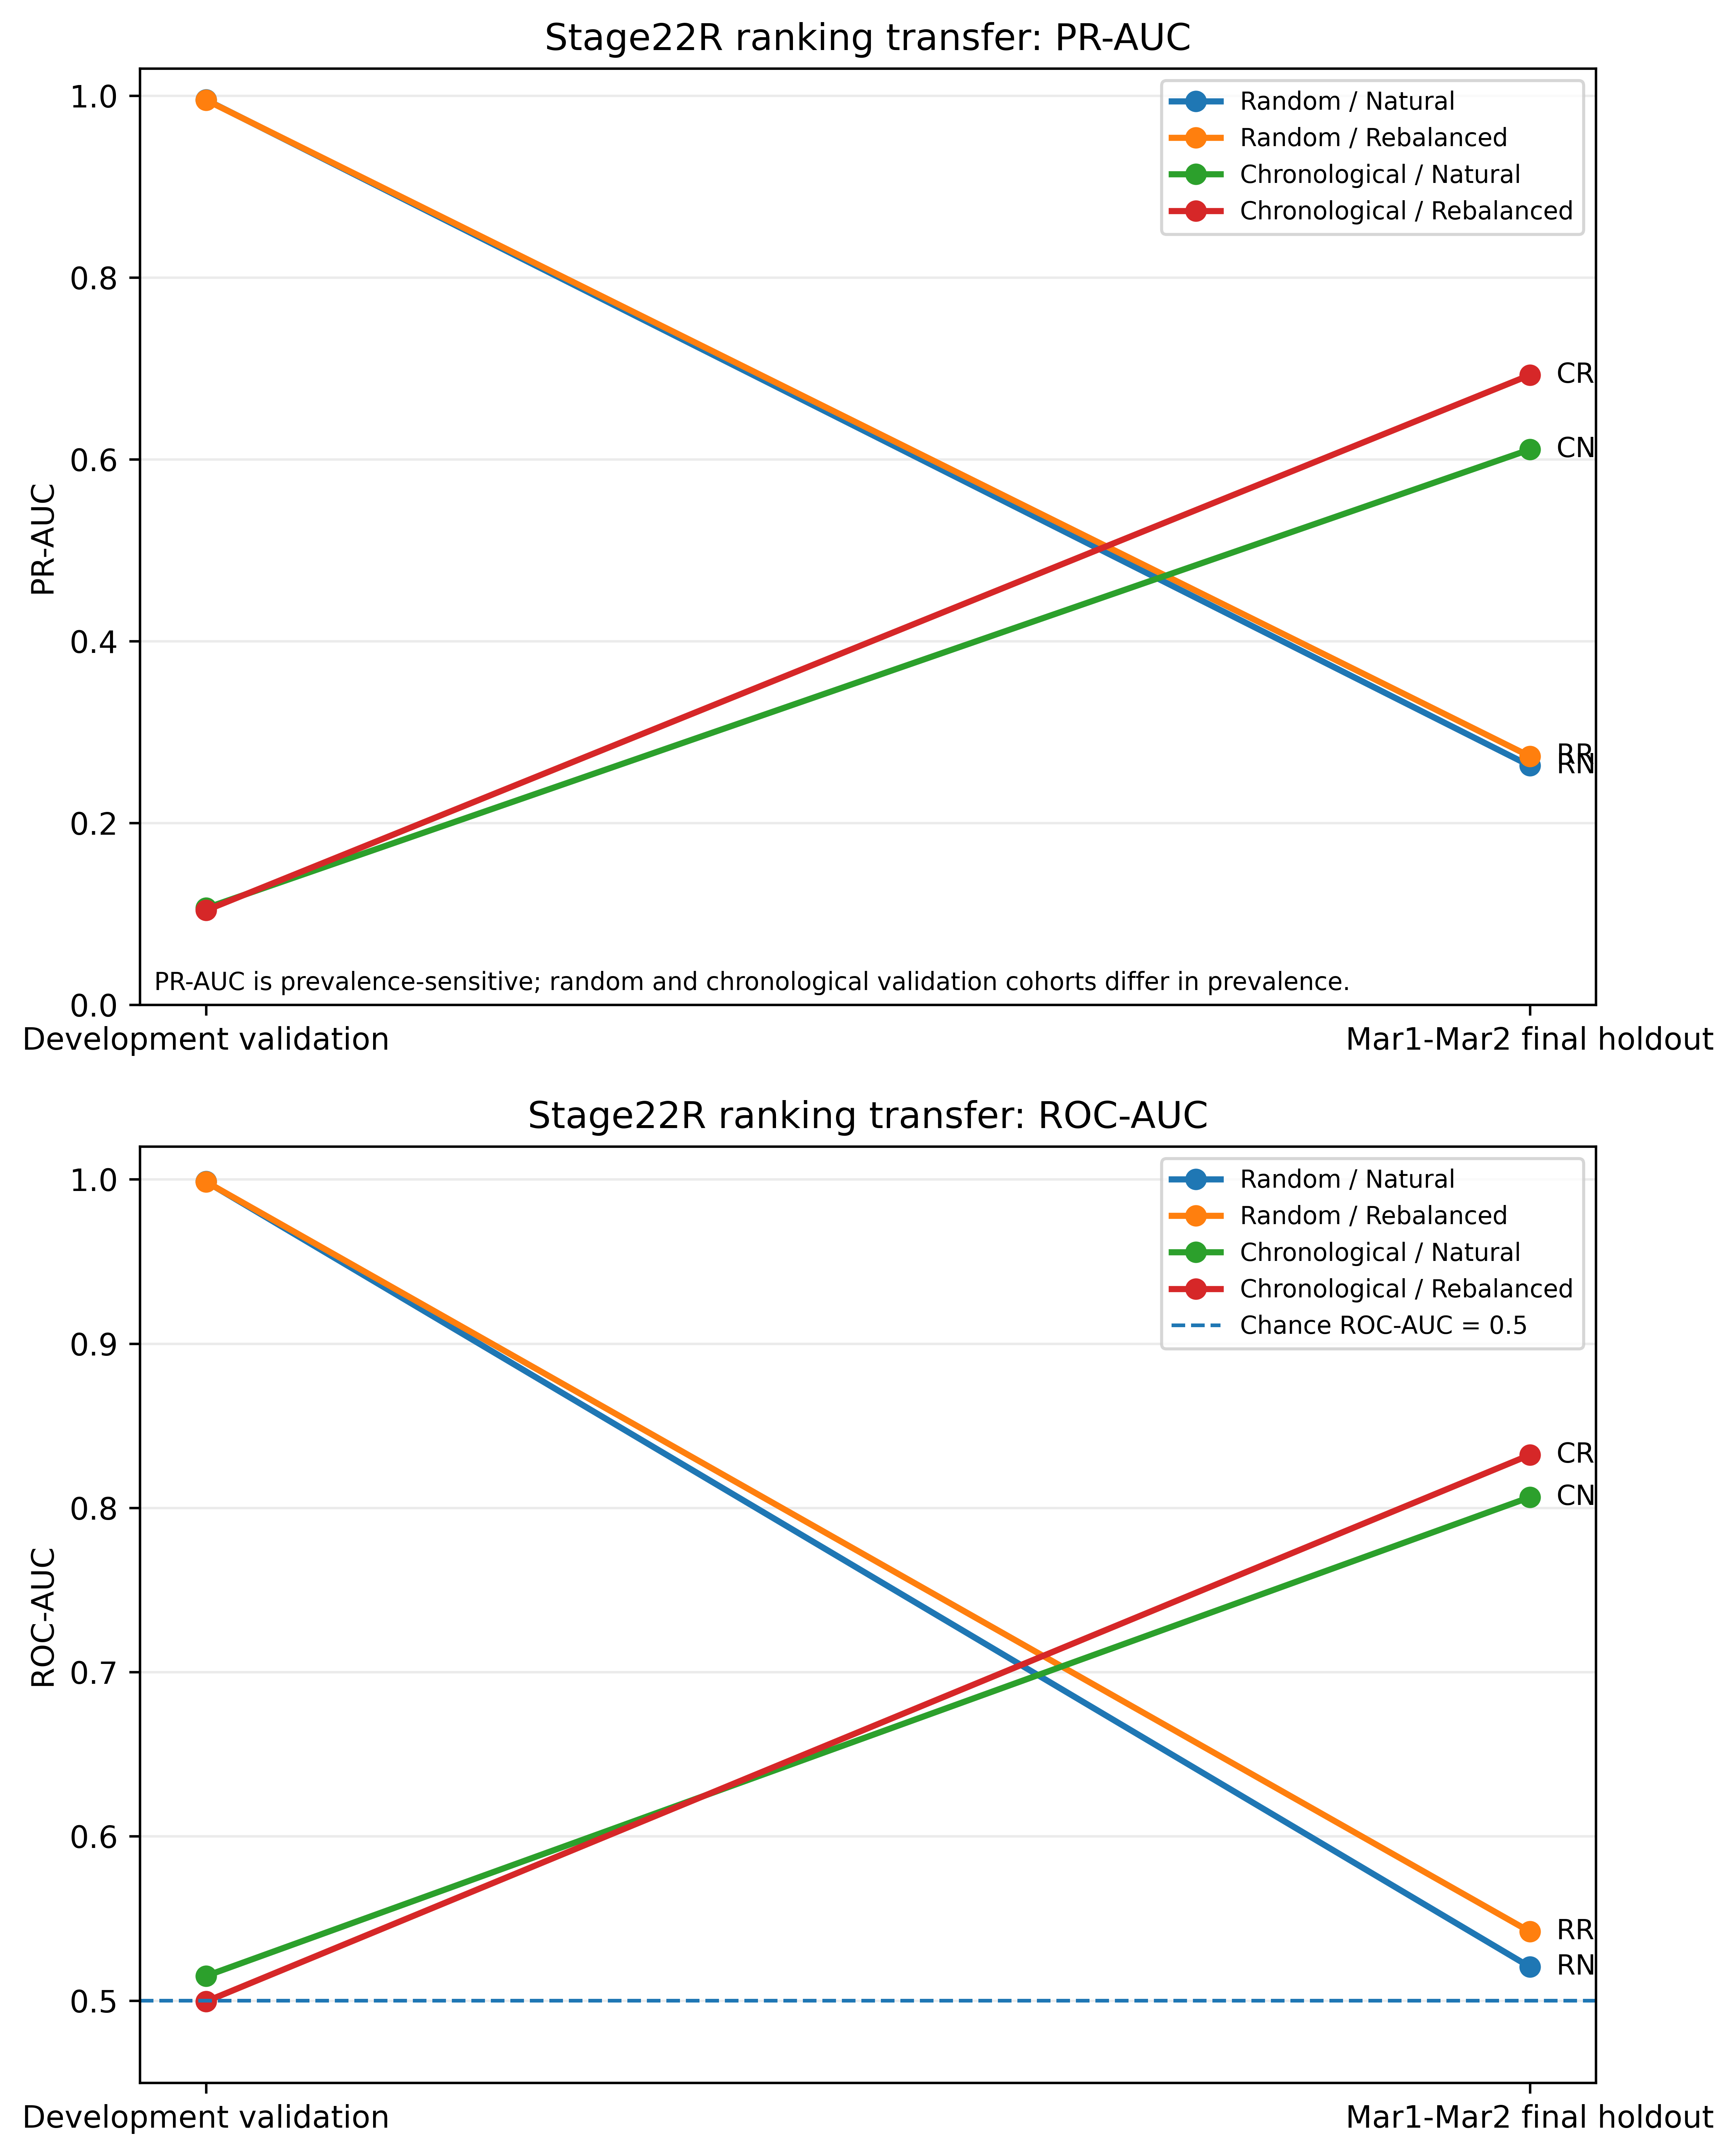
\includegraphics[width=0.95\textwidth]{figures/figure1.png}
\caption{Temporal ranking transfer on the shared forward IDS2018 target. Existing panels report (a) PR-AUC and (b) ROC-AUC for frozen random and chronological development geometries. The five-seed stability summaries establish a 5/5 descriptive ordering, not a significance test; the target was historically opened, thresholds are evaluated separately, and chronology remains entangled with family composition.}
\label{fig:1}
\end{figure}
\begin{table}[htbp]
\centering
\scriptsize
\setlength{\tabcolsep}{3pt}
\caption{Five-seed temporal stability on the shared forward target. SD is training-seed standard deviation under the frozen recipe; the directional count is descriptive over the five registered seeds.}
\begin{tabularx}{\textwidth}{@{}>{\raggedright\arraybackslash}X*{4}{>{\centering\arraybackslash}X}>{\raggedright\arraybackslash}X@{}}
\toprule
Development geometry & Mean ROC-AUC & ROC-AUC SD & Mean PR-AUC & PR-AUC SD & Directional result \\
\midrule
Random-natural & 0.5176 & 0.0073 & 0.2599 & 0.0034 & Lower than chronological in 5/5 seeds for both metrics \\
Chronological-natural & 0.8209 & 0.0085 & 0.6388 & 0.0322 & Higher than random in 5/5 seeds for both metrics \\
\bottomrule
\end{tabularx}
\end{table}

\subsection{5.3 Were shortcut and explanation conclusions stable?}
Shortcut-subset effects varied by development geometry and learner (Figure 2). The behavior-restricted representation retained strong random-split discrimination but not the chronological result, and family composition was narrower in the chronological population. Matched-size placebo removals also produced non-zero split interactions, including frozen conditional intervals excluding zero. The observed interactions therefore establish feature-set sensitivity without identifying a named feature as leakage or a causal source of transfer behavior.
Local explanations supplied a related counterexample. LIME rankings were comparatively stable across perturbation seeds, but only 2 of 64 explanations met all prespecified fidelity and cross-method criteria, and 31 of 64 failed to reproduce the model's local classification decision. Mean SHAP-LIME top-10 Jaccard agreement was 0.304 for XGBoost and 0.360 for LightGBM. Stable explanations were not necessarily faithful explanations.
\begin{figure}[htbp]
\centering
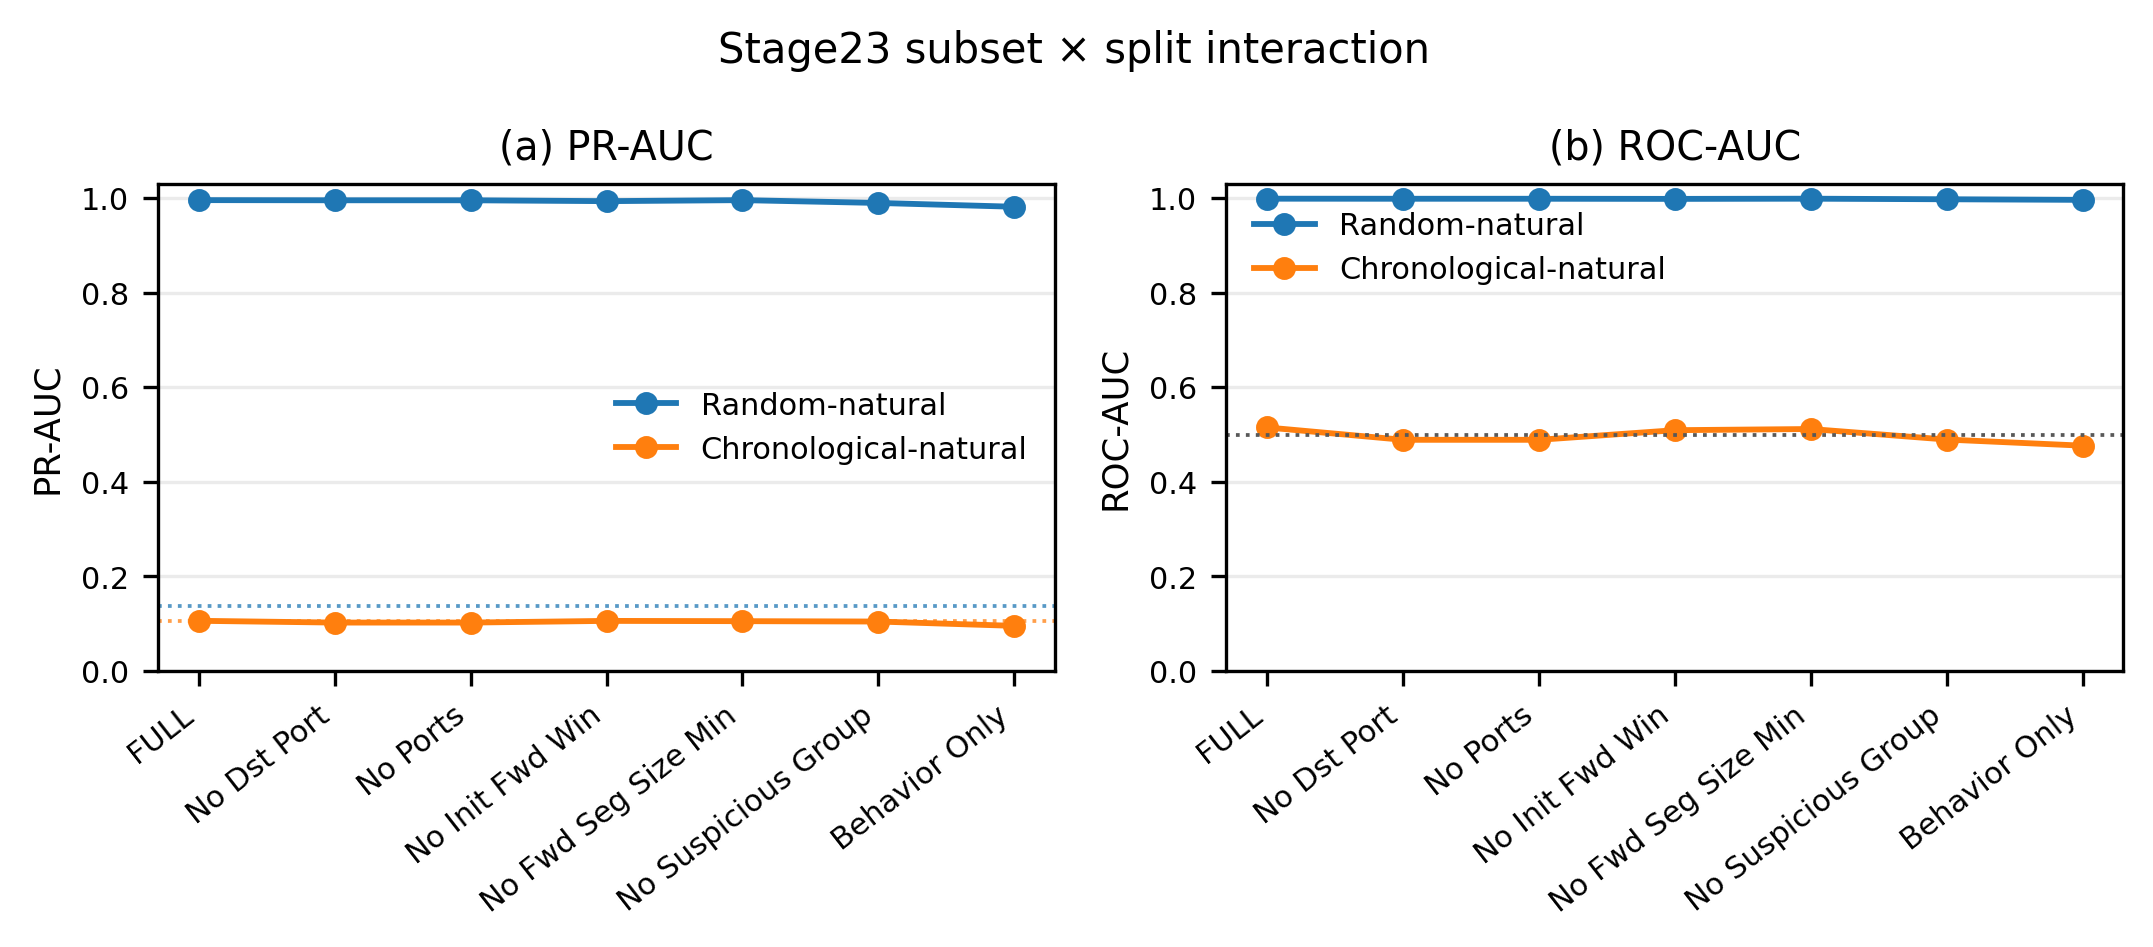
\includegraphics[width=\textwidth]{figures/fig2.png}
\caption{Shortcut-subset sensitivity by validation geometry. The approved asset reports native ranking behavior across seven frozen feature subsets, random-natural and chronological-natural splits, and the evaluated tree learners. Conditional subset effects do not identify leakage or a transfer mechanism; matched-size placebo interactions remain part of the interpretation.}
\label{fig:2}
\end{figure}

\subsection{5.4 Was cross-dataset transfer symmetric?}
Bridge62 transfer was strongly directional (Figure 3; Table 3). IDS2018-to-CICIDS2017 evaluation achieved PR-AUC 0.667483 and ROC-AUC 0.733946 on 2,830,743 effective target rows. In the reciprocal direction, target attack prevalence was 0.104847, PR-AUC was 0.108176, and ROC-AUC was 0.525167. The reverse PR-AUC was therefore close to its prevalence anchor, while the forward bridge retained substantial ranking signal.
A larger bridge did not yield one metric direction. Correcting aggregate-flag serialization in bridge70 changed PR-AUC by -0.007729, ROC-AUC by +0.002192, and Brier score by +0.005087; the frozen paired intervals excluded zero. The two \texttt{GROUNDED\_S4} cells remained cancelled because exact membership was unavailable. Neither the metric-specific sensitivity nor the missing cells are hidden by averaging the directions.
\begin{figure}[htbp]
\centering
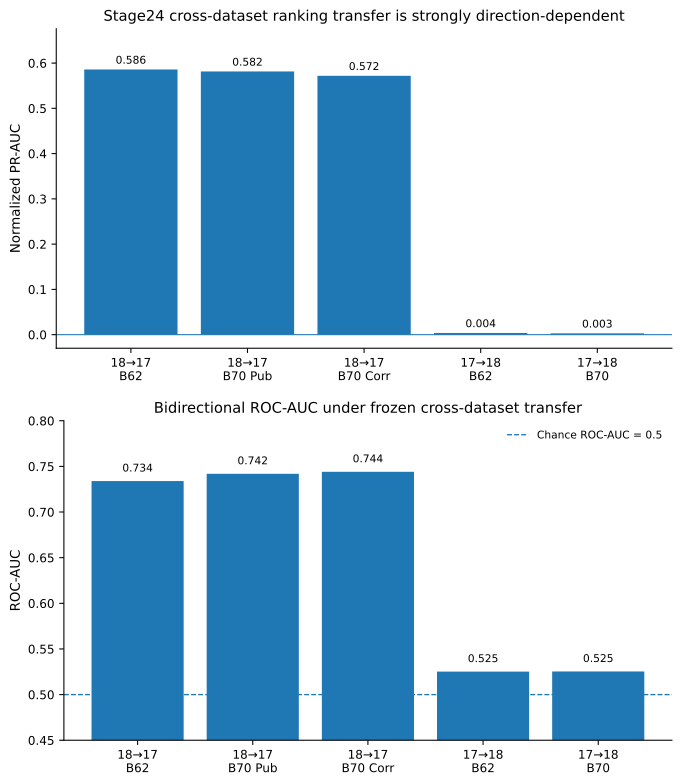
\includegraphics[width=\textwidth]{figures/figure3.png}
\caption{Bidirectional cross-dataset ranking under bridge62. Existing panels report normalized PR-AUC and ROC-AUC. Each point uses its frozen direction-specific source learner, target population, prevalence, and semantic feature contract; the panels do not define an average transfer score.}
\label{fig:3}
\end{figure}
\begin{table}[htbp]
\centering
\scriptsize
\setlength{\tabcolsep}{3pt}
\caption{Primary bidirectional bridge62 transfer. PR-AUC is interpreted against each target's attack prevalence; ROC-AUC is the direction-specific ranking metric. Different source and target protocols preclude pooling.}
\begin{tabularx}{\textwidth}{@{}>{\raggedright\arraybackslash}X>{\raggedright\arraybackslash}X*{3}{>{\centering\arraybackslash}X}@{}}
\toprule
Direction & Target scope & Target prevalence & PR-AUC & ROC-AUC \\
\midrule
IDS2018 to CICIDS2017 & 2,830,743 effective rows & Target-specific & 0.667483 & 0.733946 \\
CICIDS2017 to IDS2018 & Frozen February 28 target & 0.104847 & 0.108176 & 0.525167 \\
\bottomrule
\end{tabularx}
\end{table}

\subsection{5.5 Did projected precision imply operational utility?}
Projected PPV, workload, and yield did not align uniformly (Figure 4; Table 4). At 0.1\% assumed attack prevalence, the random-development STANDARD point retained PPV 0.965572 but required 33.5 analyst-hours per day under the frozen traffic and service-time scenario. The chronological-development STANDARD point projected PPV 0.000551068 and only 0.0322 true alerts per day: its small workload reflected negligible yield.
Directionality persisted under the same prior-shift translation. Forward STANDARD transfer points projected PPV 0.039233-0.060313, while reverse points projected 0.000257610-0.000287993. Under the frozen 1:100 relative-cost scenario, 15/24 operating points favored the model at 0.1\% prevalence and 3/24 at 0.01\%. These are analytic projections with fixed sensitivity and FPR, not observations from a security operations center.
\begin{figure}[htbp]
\centering
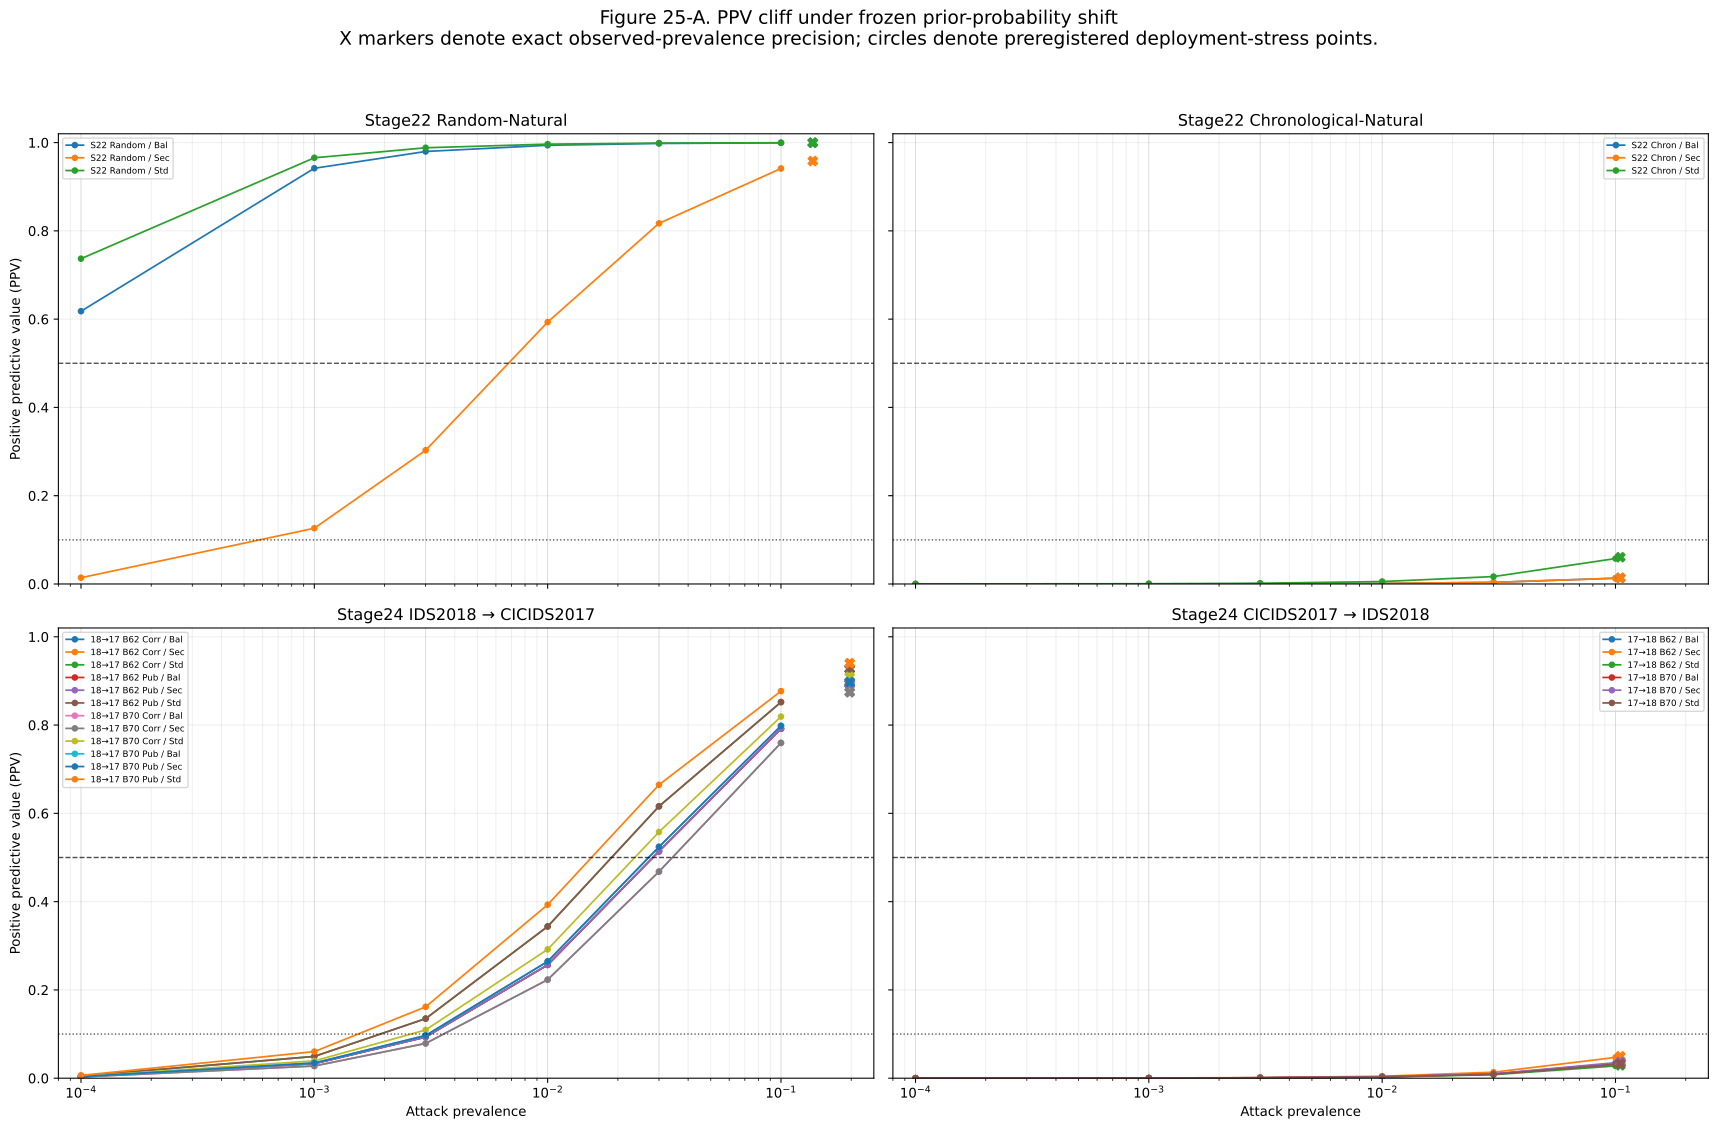
\includegraphics[width=\textwidth]{figures/figure4.png}
\caption{PPV under prevalence stress. The approved curves translate frozen true- and false-positive rates across assumed attack prevalence. PPV is positive predictive value. The prior-shift model holds conditional rates fixed; traffic, service time, capacity, and relative costs are scenario assumptions rather than field measurements.}
\label{fig:4}
\end{figure}
\begin{table}[htbp]
\centering
\scriptsize
\setlength{\tabcolsep}{3pt}
\caption{Selected operating-point translations at 0.1\% assumed prevalence. PPV and workload/yield are conditional on the frozen rates, daily traffic, and analyst service-time assumptions; STANDARD denotes the inherited standard operating role.}
\begin{tabularx}{\textwidth}{@{}>{\raggedright\arraybackslash}X>{\centering\arraybackslash}X>{\raggedright\arraybackslash}X>{\raggedright\arraybackslash}X@{}}
\toprule
Frozen condition & Projected PPV & Operational quantity & Interpretation boundary \\
\midrule
Random-development STANDARD & 0.965572 & 33.5 analyst-hours/day & High PPV does not ensure manageable workload \\
Chronological-development STANDARD & 0.000551068 & 0.0322 true alerts/day & Low workload does not ensure useful yield \\
Forward transfer STANDARD range & 0.039233-0.060313 & Direction-specific & Conditional prior-shift projection \\
Reverse transfer STANDARD range & 0.000257610-0.000287993 & Direction-specific & Conditional prior-shift projection \\
\bottomrule
\end{tabularx}
\end{table}

\subsection{5.6 Was one compute backend consistently faster?}
Backend advantage depended on architecture and measurement path (Figure 5). At batch one, the p95 CPU-over-GPU latency ratio was 1.94 for the five-checkpoint soft-voting ensemble and 1.58 for the single-resource reference, indicating a GPU advantage. Ratios of 0.16 for CatBoost and 0.26 for XGBoost indicated a CPU advantage under the same convention. The packet-image CNN ratio was 10.86, while the ViT ratio was 1.05. Unsupported LightGBM GPU execution and unavailable paths remained compatibility statuses rather than timing values.
\begin{figure}[htbp]
\centering
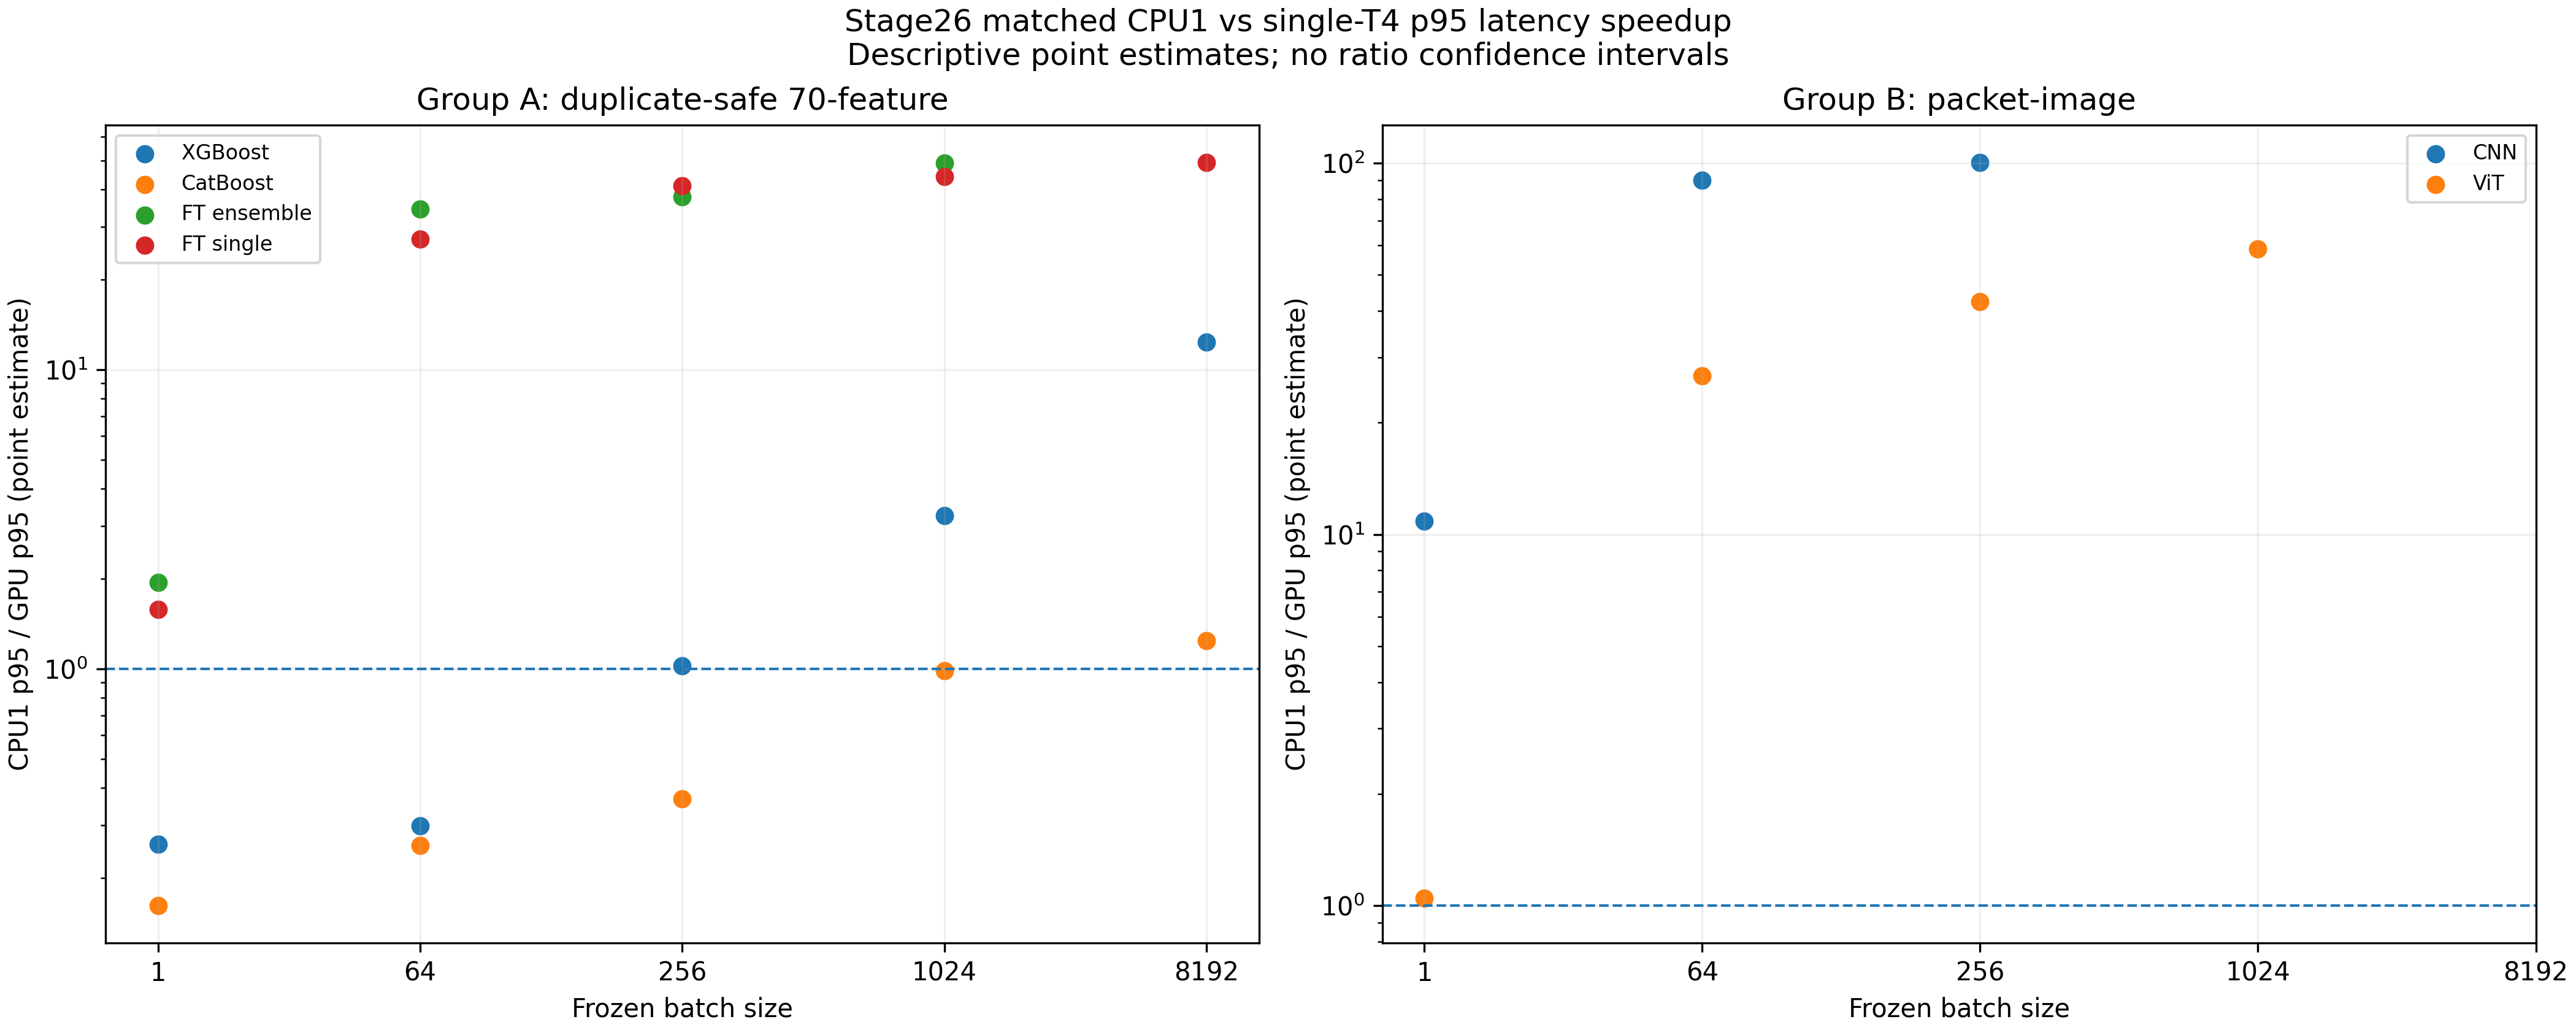
\includegraphics[width=\textwidth]{figures/fig5.png}
\caption{Hardware-specific p95 CPU/GPU comparison. The approved asset compares batch-one p95 latency ratios for compatible prepared-input-to-probability paths on the recorded hardware and software. Values are descriptive point estimates; unsupported backends, capture, flow extraction, alert aggregation, and analyst response are outside the comparison.}
\label{fig:5}
\end{figure}

\subsection{5.7 Did eligible withheld families behave uniformly?}
LOAO results were selective (Figure 6; Table 5). DDoS ranking was strong for XGBoost (ROC-AUC 0.9982; PR-AUC 0.9925) and LightGBM (ROC-AUC 0.9986; PR-AUC 0.9940). Web Attack also retained ranking for XGBoost (ROC-AUC 0.9693; PR-AUC 0.7206) and LightGBM (ROC-AUC 0.9901; PR-AUC 0.7605).
Other families were more conditional. Bot produced XGBoost ROC-AUC 0.3224 and PR-AUC 0.003256 but LightGBM ROC-AUC 0.5591. Port Scan ROC-AUC was 0.5506 for XGBoost and 0.7559 for LightGBM. Infiltration remained descriptive at 36 positives, and DOS and AUTH\_BRUTE\_FORCE were ineligible rather than model failures. Ranking and frozen-threshold recall could also disagree, so no pooled novelty score was formed.
\begin{figure}[htbp]
\centering
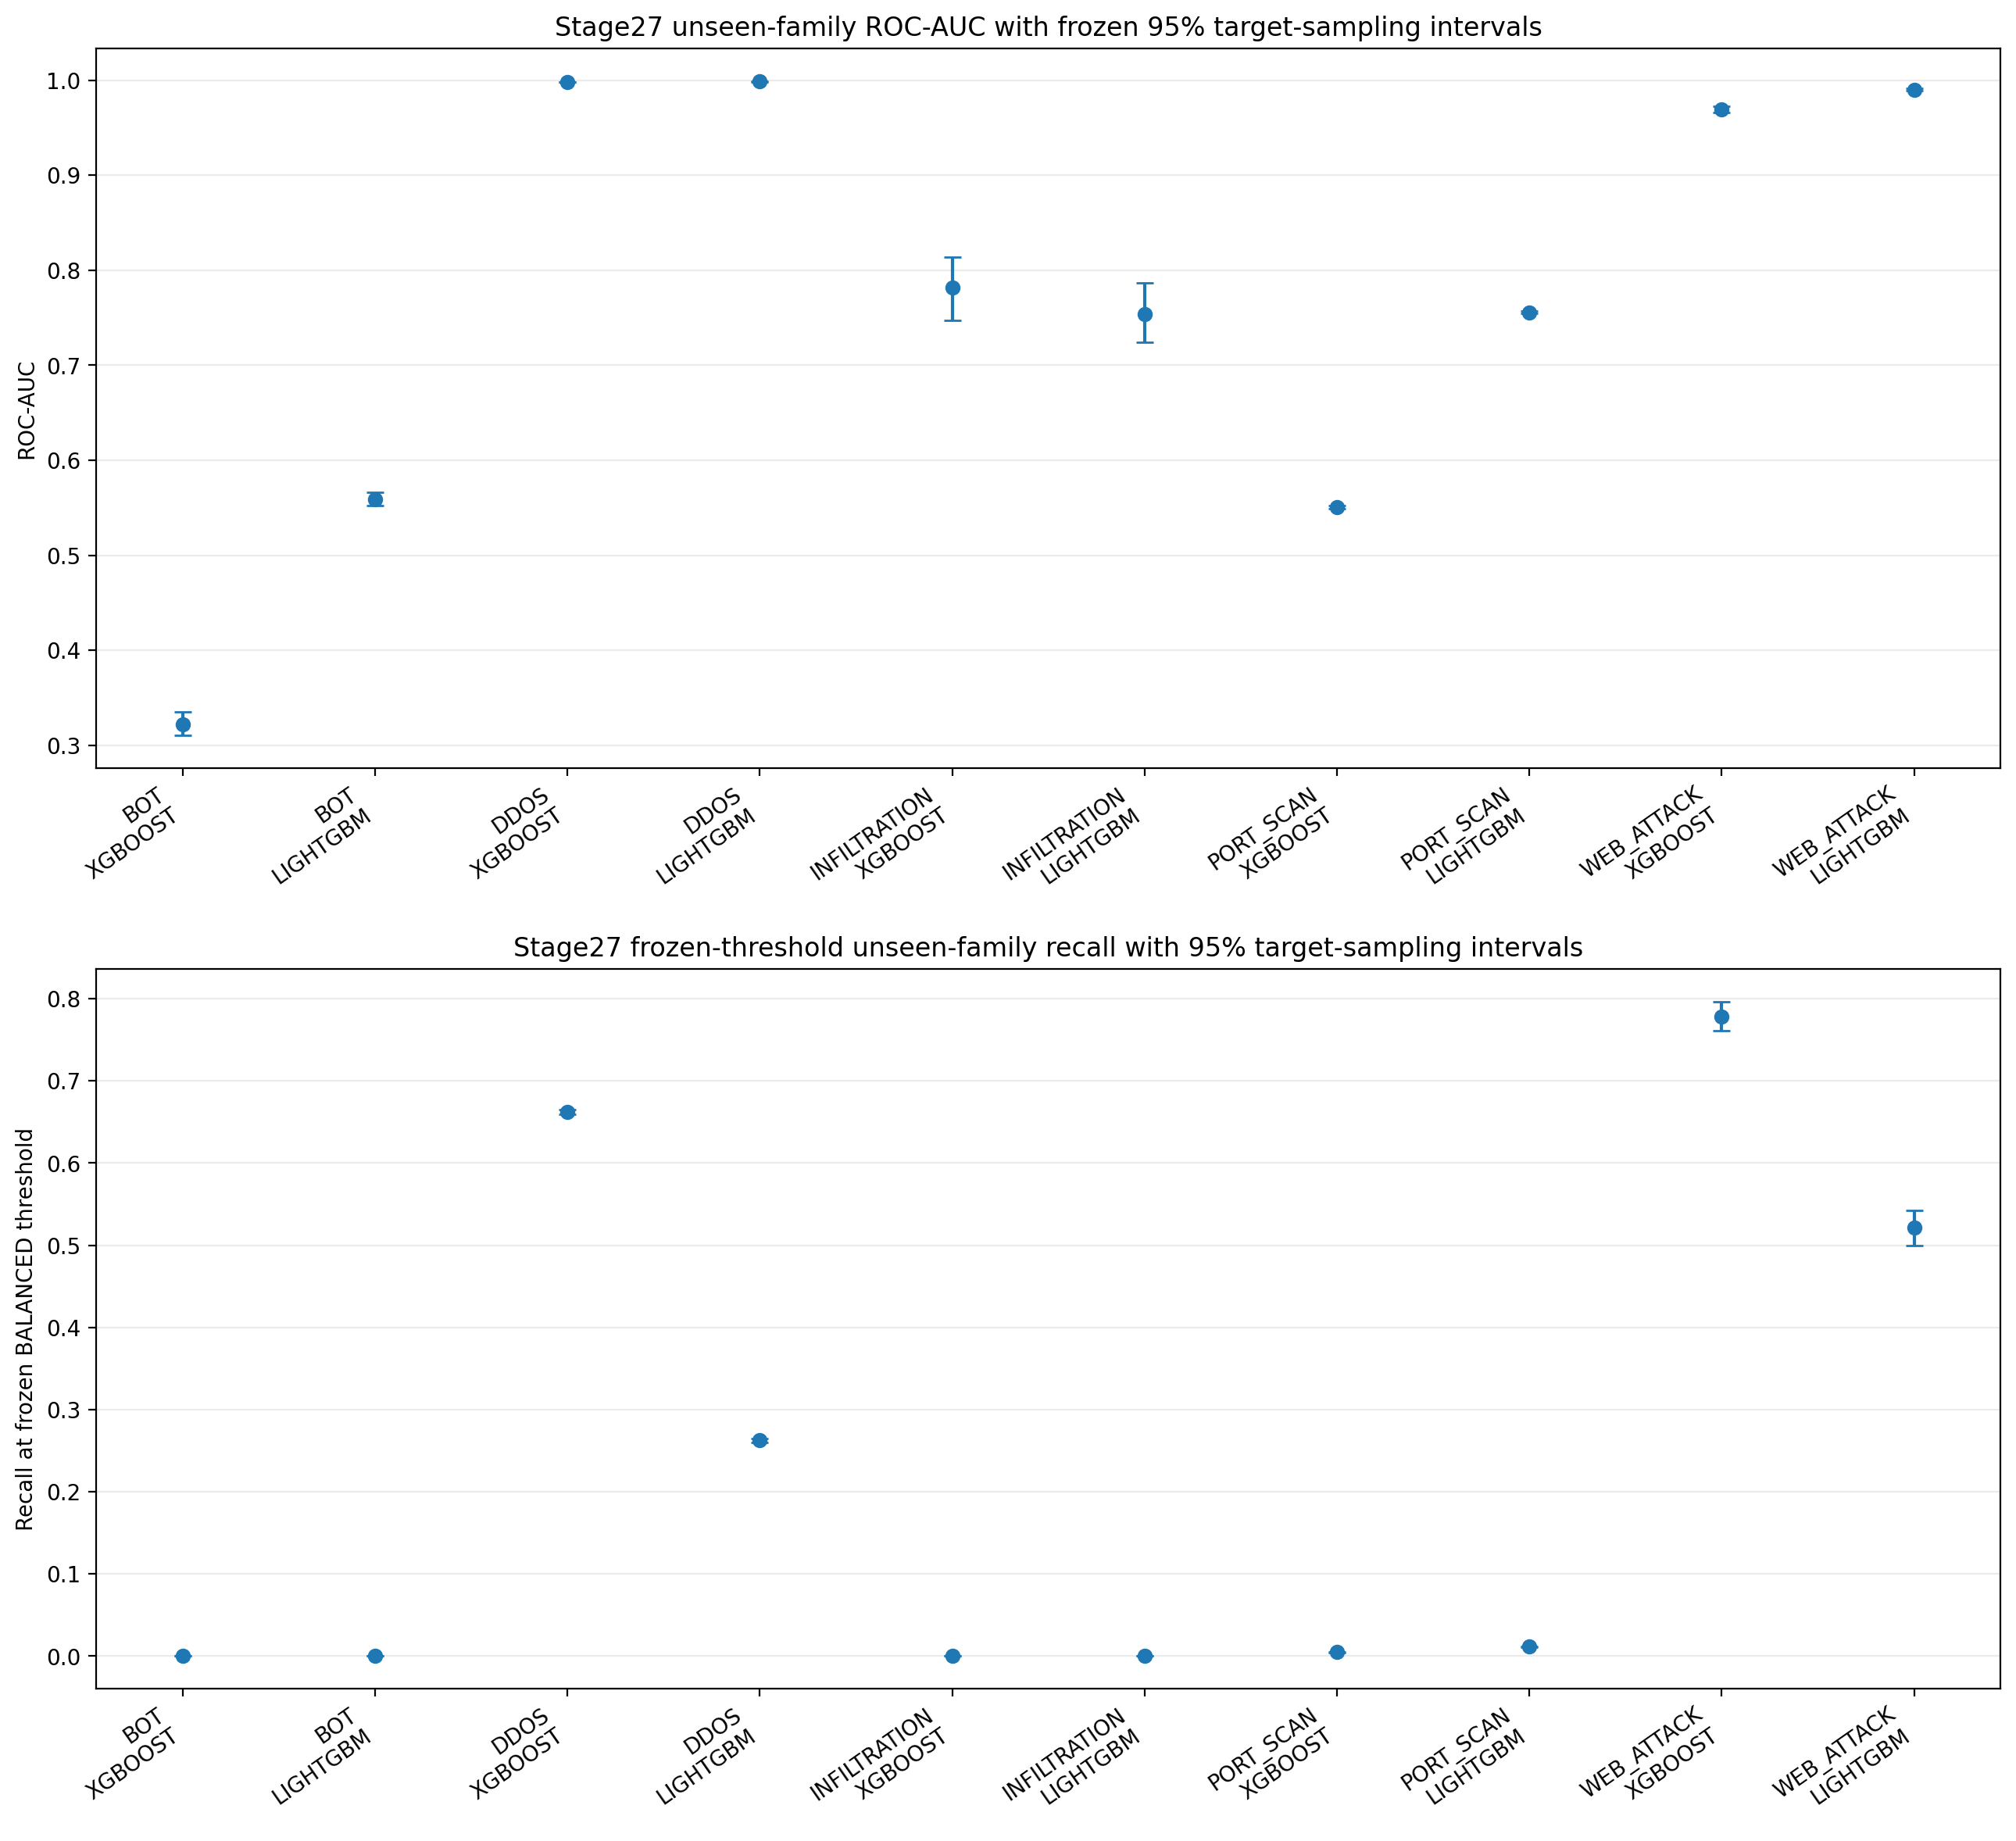
\includegraphics[width=\textwidth]{figures/figure6.png}
\caption{Eligible-family ranking and balanced-threshold recall. Existing panels report ROC-AUC with frozen conditional intervals and balanced-threshold recall for separate eligible families and learners. Infiltration is descriptive at support 36; ineligible families are absent; the panels do not constitute an aggregate future-attack score.}
\label{fig:6}
\end{figure}
\begin{table}[htbp]
\centering
\small
\caption{Frozen conclusion-stability classification for eligible families. Classifications combine family-specific ranking, frozen-threshold behavior, support, learner contrast, and the five-seed stability rules; they are not pooled metrics.}
\begin{tabularx}{\textwidth}{@{}>{\raggedright\arraybackslash}X>{\raggedright\arraybackslash}X>{\raggedright\arraybackslash}X@{}}
\toprule
Family & Frozen synthesis & Required qualification \\
\midrule
DDoS & Strong ranking for both learners & Eligible benchmark family only \\
Web Attack & Ranking retained for both learners & Magnitude and thresholds remain learner-specific \\
Port Scan & Qualitative conditions retained across seeds & Ranking magnitude is learner-dependent \\
Bot & Learner-dependent & Frozen-threshold detection remains weak \\
Infiltration & Descriptive only & Held-out positive support is 36 \\
\bottomrule
\end{tabularx}
\end{table}

\subsection{5.8 Did central conclusions survive the frozen realizations?}
All 108/108 preregistered new fits in the frozen stability program completed, with 12 artifacts reused as declared and no planned execution outstanding. Completion did not enlarge inferential scope: no best seed was selected, seed variation was not combined with bootstrap uncertainty, and the shared temporal target remained historically opened.
The chronological-over-random ranking direction held in all evaluated seeds. DDoS, Port Scan, and Web Attack met the registered qualitative conditions for both learners; Bot remained learner-dependent and Infiltration descriptive. Random LOAO controls were mixed and family-specific. The controls support an interaction between novelty difficulty and chronology in some comparisons but do not identify one mechanism.

\subsection{5.9 What survived across the validation axes?}
Table 6 synthesizes the frozen chain without treating unlike quantities as commensurable. Strong benchmark discrimination, chronological forward ranking, forward bridge signal, selected family transfer, and compatible computational paths survived within their declared scopes. Frozen thresholds, symmetric portability, simple shortcut causality, universal operational preference, and uniform family conclusions did not.
\begin{table}[htbp]
\centering
\scriptsize
\setlength{\tabcolsep}{2pt}
\renewcommand{\arraystretch}{0.82}
\caption{Integrated native-metric validity matrix. Each row preserves its population, metric family, and interpretation ceiling. The table summarizes frozen evidence and is not a normalized degradation, generalization, or composite performance score.}
\begin{tabularx}{\textwidth}{@{}>{\raggedright\arraybackslash}X*{4}{>{\raggedright\arraybackslash}X}@{}}
\toprule
Validity axis & Principal observation & What survived & What remained conditional or unsupported & Claim ceiling \\
\midrule
Benchmark/\allowbreak reference & Strong F1 and ranking on the processed split & Within-reference discrimination & Inference to chronology, transfer, or deployment & Processed reference only \\
Duplicate/split & Frozen memberships and target roles were auditable & Explicit role separation & Latent-session independence & Traceable memberships only \\
Temporal & Chronological ranking exceeded random ranking across five seeds & Directional ranking contrast & Threshold transfer and sole mechanism & Evaluated chronology and recipe \\
Shortcut & Subset effects depended on split and learner; placebos interacted & Representation sensitivity & Universal removal benefit or causal leakage & Preregistered subsets and controls \\
Cross-dataset & Forward ranking signal contrasted with near-baseline reverse transfer & Direction-specific forward signal & Symmetry, arbitrary datasets, cancelled cells & Frozen bridges and targets \\
Prevalence/\allowbreak operational & PPV, workload, yield, and cost preference diverged & Assumption-explicit translation & Field performance or universal preference & Frozen prior-shift scenarios \\
Computational & Backend advantage varied by compatible model path & Measured component feasibility & Unsupported paths and end-to-end cost & Recorded hardware/software \\
Unseen family & Several families transferred; others depended on learner or support & Selected eligible-family capability & Uniform future-attack detection & Eligible benchmark families \\
Seed/control & Central directions survived selected seeds; controls were mixed & Finite-realization stability & Population guarantee or one causal account & Frozen seed registry \\
\bottomrule
\end{tabularx}
\end{table}

\section{Discussion}

\subsection{6.1 Stronger validation changed the claim, not every result}
The reference experiment remains a credible answer to a narrow question: selected tree ensembles discriminated the processed holdout labels well under frozen validation choices. Stronger validation did not erase that arithmetic or make benchmark evaluation uninformative. Instead, each axis changed the population, operating rule, representation, or resource assumption to test a broader inference.
The resulting pattern was not monotonic. Chronological development retained substantially stronger forward ranking than random development. The forward semantic bridge retained cross-dataset signal, DDoS and Web Attack remained discriminable when withheld, and compatible model paths were feasible on the measured system. Other findings were less favorable: frozen thresholds transferred poorly, reverse cross-dataset ranking was near its anchor, and some family outcomes depended on learner or support. Benchmark performance is therefore a property of one evaluation system. A broader capability claim must name the additional condition under which it was validated.

\subsection{6.2 Temporal, shortcut, and explanation evidence constrain mechanism claims}
The temporal evidence separates ranking from score-scale transfer. Chronological development ranked the shared forward population more effectively in every frozen realization, yet its inherited thresholds almost never fired. This does not show that chronological development is universally preferable. It shows that validation geometry can change both ranking and operating behavior. Family-aware controls remain mixed, so chronology or drift alone cannot explain the contrast.
Shortcut controls reinforce that restraint. Named removals altered results, but matched placebos also interacted with split geometry. Chronological family composition also differed from random composition. The study can report subset sensitivity without treating a field as proven leakage or as the cause of domain transfer. LIME provides a related warning: perturbation rankings could be stable while local decision reconstruction and cross-method fidelity failed. Explanation reports should measure fidelity and agreement rather than equate repeatability with validity.

\subsection{6.3 Transfer is directional and threshold utility is a separate decision}
The bidirectional bridge makes dataset portability a source-to-target statement. IDS2018-trained models retained useful ranking on CICIDS2017 under bridge62, while the reciprocal evaluation was close to its target anchor. The directions use different source learners, prevalence, collection periods, and target roles. Averaging them would remove the finding. Metric-specific responses to the aggregate-flag correction also show that a larger feature intersection is not automatically a better semantic bridge. The cancelled cells preserve another boundary: exact membership governance can leave a planned comparison unestimable.
Ranking and operating utility also diverged across temporal, cross-dataset, and LOAO results. ROC-AUC and PR-AUC integrate score order across thresholds; precision, recall, F1, and FPR describe one selected point. A transported ranking can coexist with an unsuitable threshold when score scale or prevalence changes. Prospective recalibration might be useful, but it would require new governed data and evaluation. Target-guided recalibration was not performed here.

\subsection{6.4 Operational projections and compute profiles answer different questions}
Prior-shift translation demonstrates that PPV alone does not determine workflow. Under the frozen scenarios, high projected PPV coexisted with analyst demand exceeding one day, while low demand could result from almost no true detections. Relative-cost preference also changed with assumed prevalence. Evaluation protocols should report the inherited rates and the assumed prevalence, traffic, service time, capacity, and error costs. An operating point should not be labeled operationally useful from PPV alone.
The profiling analysis asks a complementary systems question: can a compatible prepared-input-to-probability path run in the declared environment? CPU/GPU advantage varied by model family, and unsupported paths remained statuses. These measurements neither validate PPV nor cover capture-to-alert latency. Operational analysis and computational profiling belong in the same decision chain, but their evidence boundaries remain separate.

\subsection{6.5 Withheld-family evidence must remain heterogeneous}
Zero exposure during training and validation did not produce one family outcome. DDoS and Web Attack transferred strongly across learners. Port Scan retained qualitative stability but differed in magnitude, and Bot was learner-dependent. Infiltration remained descriptive, while two families were ineligible. One novelty score would hide these differences in support, threshold behavior, and learner dependence.
This heterogeneity is informative. Strong family results prevent a universal negative conclusion. Weak and ineligible cases prevent a universal positive one. A withheld benchmark family can share infrastructure, extraction cues, or behavior with known classes; it is not equivalent to an arbitrary future exploit. Future evaluations should preregister eligibility, retain family support, report ranking and frozen-threshold behavior separately, and distinguish descriptive from inferential outcomes.

\subsection{6.6 An Eight-Item Validation Checklist}
The evidence supports eight claim checks. Each check uses its own metrics and controls; completing the list is not a universal guarantee of deployment validity.
\begin{enumerate}
\item \textbf{Define the reference population} Report sampling, prevalence, duplicate handling, and split construction. Use membership counts and class support as the native evidence, and state which population the resulting metrics describe.
\item \textbf{Test temporal validity} Use forward or chronological separation when it matches the intended claim. Report ranking metrics and operating-point metrics separately, and retain controls for changes in family composition or other competing mechanisms.
\item \textbf{Probe shortcut sensitivity} Ablate suspicious features and, where appropriate, compare behavior-restricted representations. Pair named interventions with negative or matched-placebo controls; an effect establishes sensitivity, not leakage or causality.
\item \textbf{Evaluate cross-dataset transfer bidirectionally} Declare the semantic feature bridge and report each source-to-target direction separately. Prohibit target adaptation or identify it explicitly, and do not average asymmetric transfer away.
\item \textbf{Stress prevalence assumptions} State the target prevalence and translate frozen rates into PPV, alert volume, and workload. Distinguish an analytic prior-shift projection from measured field performance and disclose traffic, service-time, capacity, and cost assumptions.
\item \textbf{Profile the declared deployment boundary} Report latency or throughput with the hardware, software, batch, and timed component. Include feature-extraction cost when measured; otherwise state that it is outside the boundary, along with unsupported runtime paths.
\item \textbf{Test unseen-family behavior with eligibility controls} Verify zero training and validation exposure to the held-out family, publish eligibility criteria and support, and report ranking and frozen-threshold behavior separately. Keep low-support families descriptive.
\item \textbf{Test realization stability} Repeat critical conclusions across registered seeds or model realizations without selecting the best run. Report realization spread separately from bootstrap or target-sampling uncertainty.
\end{enumerate}
These checks are modular. The appropriate subset depends on the claim, population, and intended use, and no item substitutes for another validity axis. Claim-to-artifact links should record the frozen decision, evidence source, and interpretation ceiling for each completed check.

\section{Limitations}
The governed limitations fall into six conceptual groups. The complete limitation-to-claim-ceiling matrix is provided with the supplementary and repository materials.

\subsection{7.1 Dataset and benchmark scope}
The evidence covers two related benchmark families, CSE-CIC-IDS2018 and CICIDS2017, rather than current operational networks (\texttt{LIM29-001}). The processed reference is rebalanced and stratified, so its high metrics do not establish natural-prevalence, session, temporal, or deployment validity (\texttt{LIM29-002}). Some raw data and historical scientific artifacts are unavailable or intentionally closed (\texttt{LIM29-015}). The graph result is restricted to one authenticated source and cannot establish unseen-host or full-reference capability (\texttt{LIM29-016}). The CNN/ViT comparison is a single descriptive contrast, not evidence of general architecture superiority (\texttt{LIM29-017}).

\subsection{7.2 Temporal and family-composition confounding}
Chronological memberships also change attack-family composition. Mixed controls therefore prevent attribution of the temporal contrast to chronology or concept drift alone (\texttt{LIM29-003}). The stability analysis reuses the historically opened shared target; it strengthens the frozen conclusion across realizations but is not an independent blind replication (\texttt{LIM29-018}).

\subsection{7.3 Cross-dataset and family-support constraints}
Cross-dataset conclusions depend on bridge62/70 semantics, preprocessing, learners, direction, and target roles; they do not establish bridge-independent or symmetric portability (\texttt{LIM29-004}). Two \texttt{GROUNDED\_S4} cells were cancelled because exact membership was unrecoverable, so not every planned sensitivity was executed (\texttt{LIM29-005}). LOAO coverage is also incomplete: DOS and AUTH\_BRUTE\_FORCE were structurally ineligible (\texttt{LIM29-006}), and Infiltration remains descriptive at 36 held-out positives (\texttt{LIM29-007}). These constraints preclude uniform conclusions across datasets or attack families.

\subsection{7.4 Statistical and realization uncertainty}
Paired confidence intervals are conditional on the frozen target samples, fitted models or arrays, and implementations; they do not describe unconditional deployment uncertainty (\texttt{LIM29-008}). Five registered seeds assess a fixed recipe without repeating full hyperparameter optimization. The 5/5 ordering is descriptive, not a significance test or population guarantee (\texttt{LIM29-009}).

\subsection{7.5 Operational and hardware assumptions}
The prior-shift analysis holds true- and false-positive rates fixed while prevalence changes. It measures sensitivity to that assumption, not performance under simultaneous covariate, protocol, topology, user, or attacker shift (\texttt{LIM29-012}). Traffic, analyst time, capacity, and relative costs are scenarios rather than organization-specific measurements (\texttt{LIM29-013}). Profiling covers compatible inference components on one hardware/software environment and omits complete capture-to-alert processing (\texttt{LIM29-011}). It cannot establish universal workload, economic value, latency, throughput, energy, or end-to-end cost.

\subsection{7.6 Historical reproducibility}
Some dependencies and execution environments remain\linebreak{} \texttt{VERSION\_NOT\_PROVEN}; bit-for-bit reconstruction of every historical environment is unsupported\linebreak{} (\texttt{LIM29-010}). Static provenance, scalar evidence, configurations, archives, and equivalence tests make the manuscript chain auditable, but missing data and closed artifacts prevent some end-to-end reruns (\texttt{LIM29-014}). The repository therefore supports claim-level traceability, not complete local regeneration of every result.

\section{Conclusion}
A processed benchmark score is a necessary reference, not a complete capability claim. Strong reference discrimination survived the evaluated validation chain. Chronological development retained higher forward ranking across five seeds, the forward cross-dataset bridge retained signal, and several eligible withheld families remained discriminable. Compatible inference paths were also feasible on the recorded hardware.
Other conclusions remained conditional. Frozen thresholds transferred poorly even when ranking survived. Reverse cross-dataset transfer was near its anchor. Shortcut and placebo interactions did not isolate one mechanism, operational projections depended on prevalence and workload assumptions, and withheld-family behavior varied by learner and support.
Future evaluations should name the validity condition, population, metric, operating rule, uncertainty, and adaptation boundary attached to each claim. Benchmark, temporal, shortcut, domain, operational, computational, unknown-family, and realization evidence should remain separate. This preserves failures as well as non-collapse findings. The resulting account states which capability was observed, where it survived, and what the evidence does not establish.
Stronger validation narrows or qualifies a claim; it does not require a monotonic performance decline. It also does not justify a single failure label or a universal deployment verdict.

\bibliographystyle{elsarticle-num}
\bibliography{references}
\end{document}
